\section{Ginger}
\label{sec:ginger}

\begin{spice}\label{spice:ginger}
\textsc{Ginger} \hfill \href{https://powo.science.kew.org/taxon/798372-1}{POWO} \\
\textbf{English:} \textit{ginger}. 
\textbf{Arabic:} {\arabicfont{زنجبيل}} \textit{zanjabīl}. 
\textbf{Chinese:} {\tradchinesefont{薑}} \textit{jiāng}. 
\textbf{Hungarian:} \textit{gyömbér}.  \\
\noindent{\color{black}\rule[0.5ex]{\linewidth}{.5pt}}
\begin{tabular}{@{}p{0.25\linewidth}@{}p{0.75\linewidth}@{}}
Plant species: & \taxonn{Zingiber officinale}{Roscoe} \\
Family: & \textit{Zingiberaceae} \\
Plant part used: & rhizome \\
Region of origin: & India \\
Cultivated in: & India, Jamaica, Nigeria, Sierra Leone \\
Color: & light yellow when fresh, beige when powdered \\
\end{tabular}
\end{spice}

\begin{figure}[!ht]
	\vspace{-4ex}
	\centering
	\subfloat[\centering a]{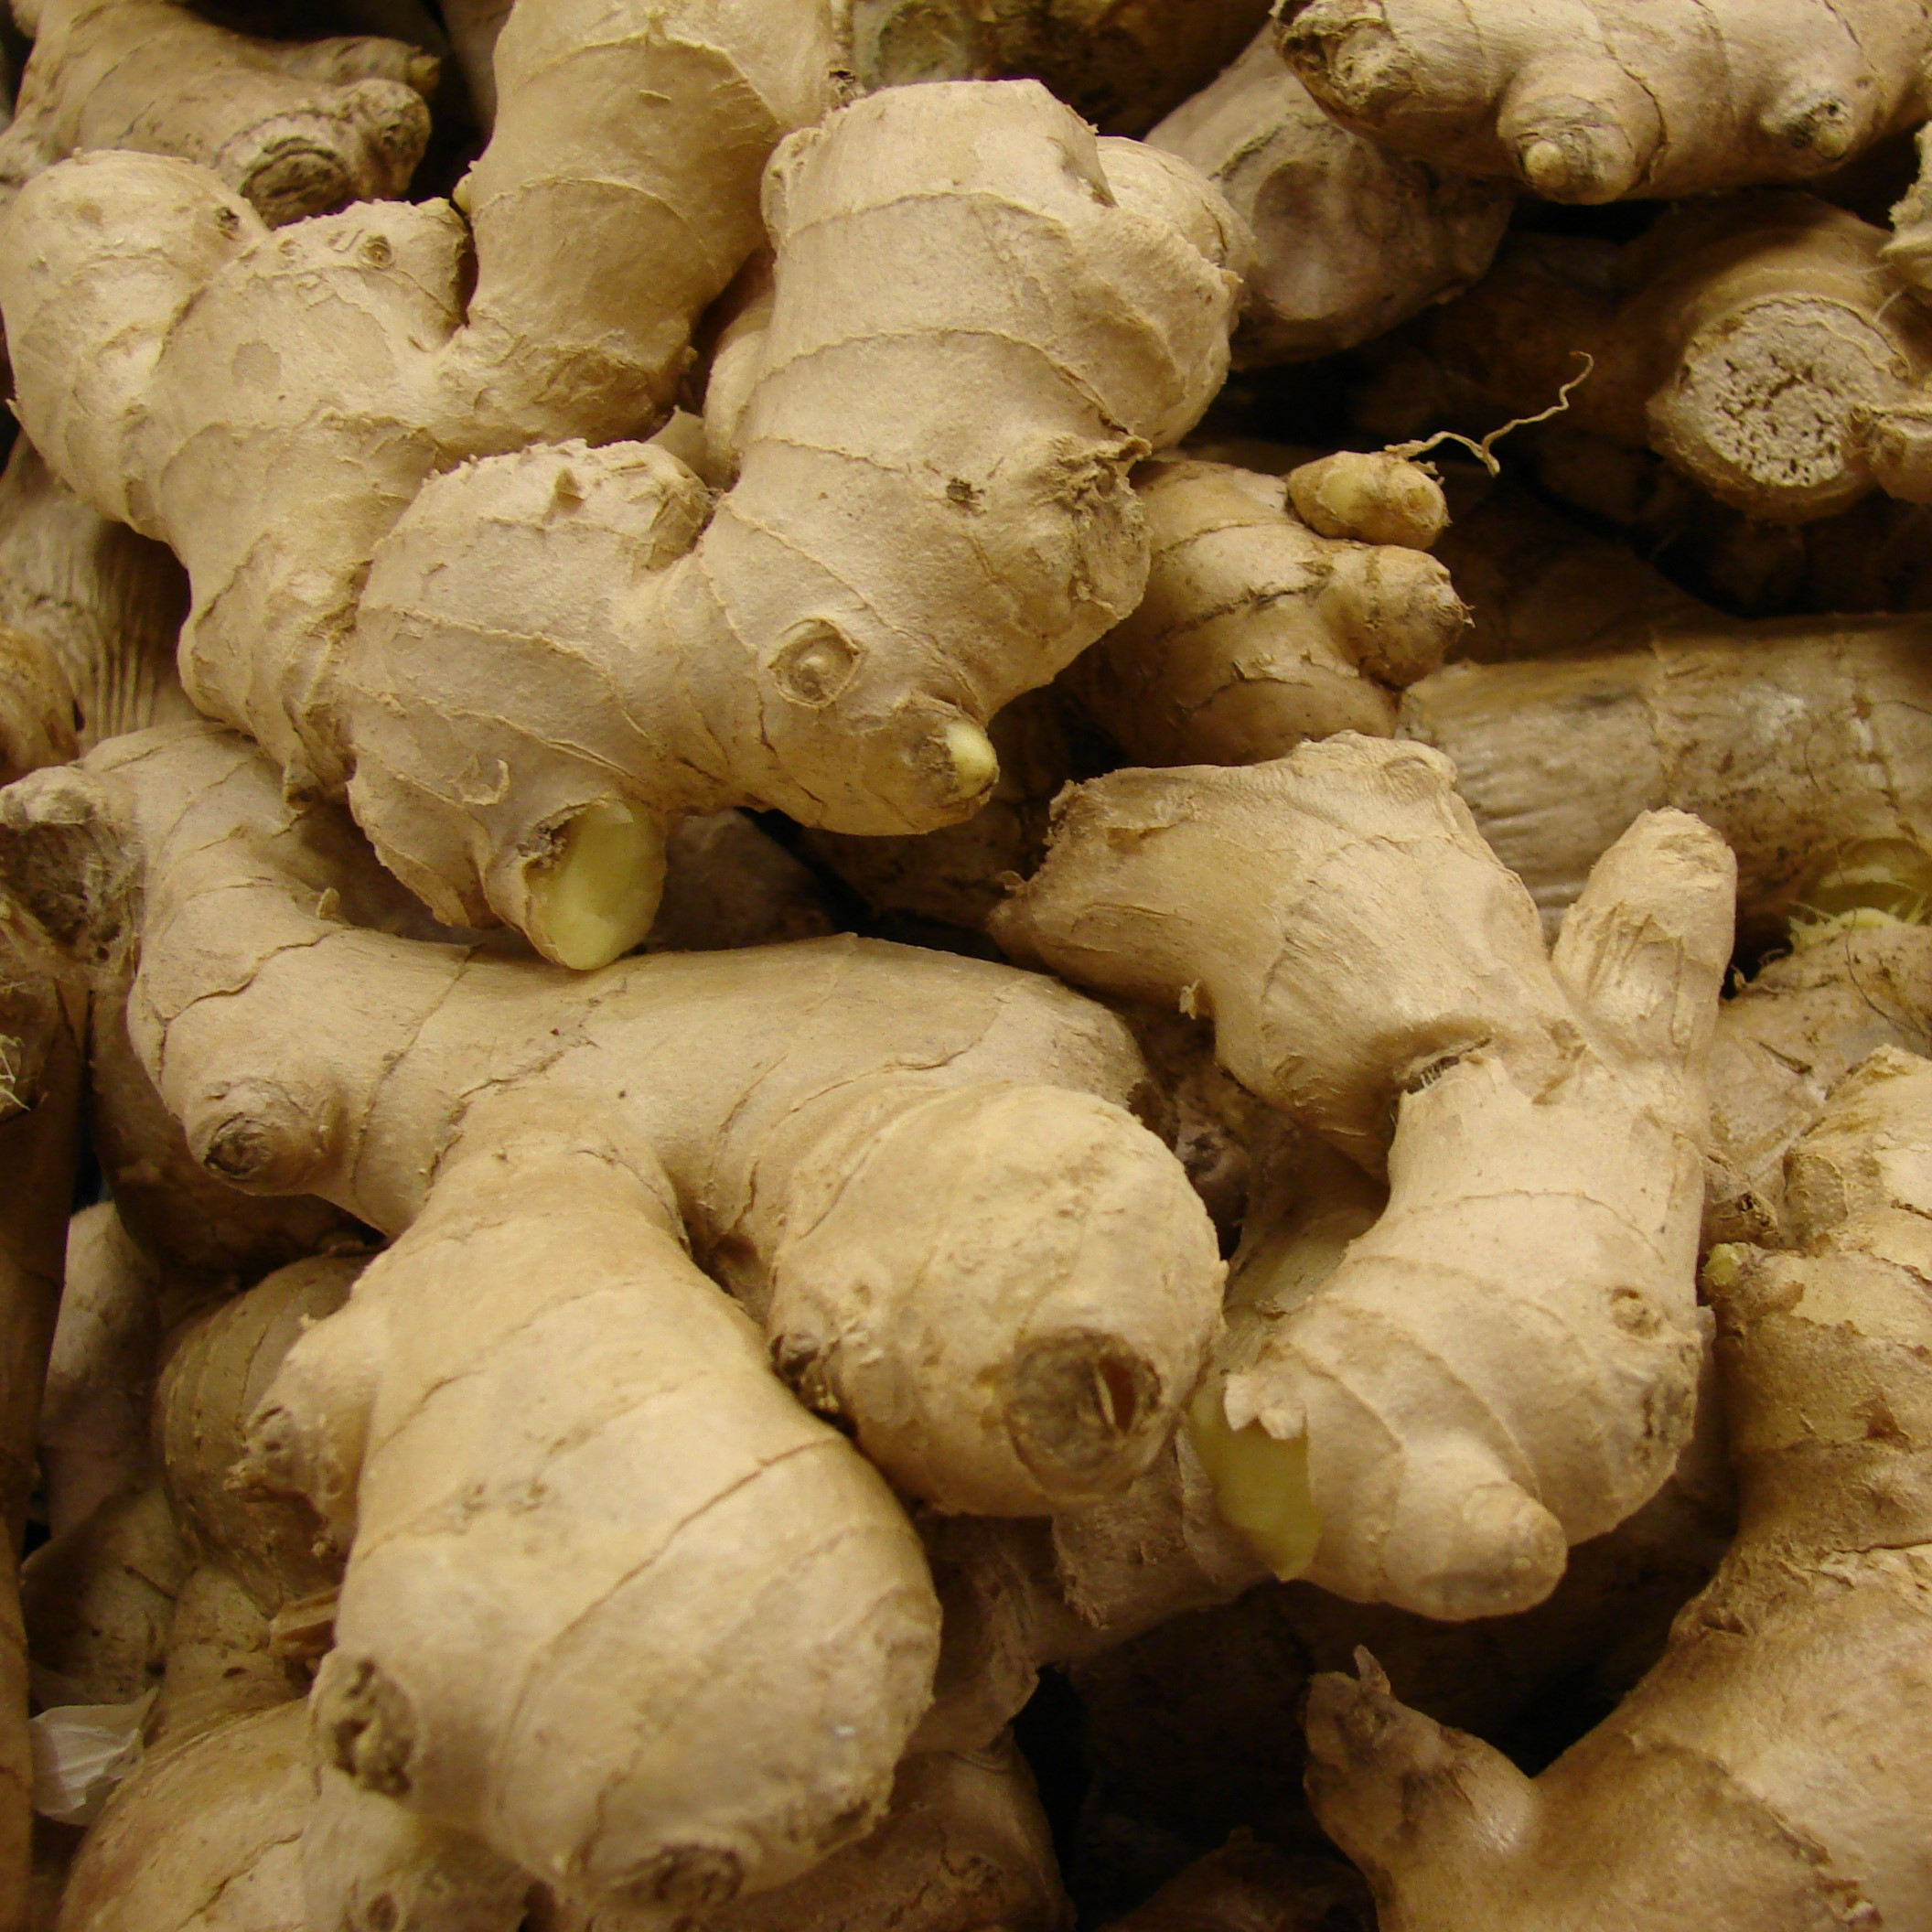
\includegraphics[width=0.3\linewidth]{imgs/spices/ginger-1.jpg}}
	\hfill
	\subfloat[\centering b]{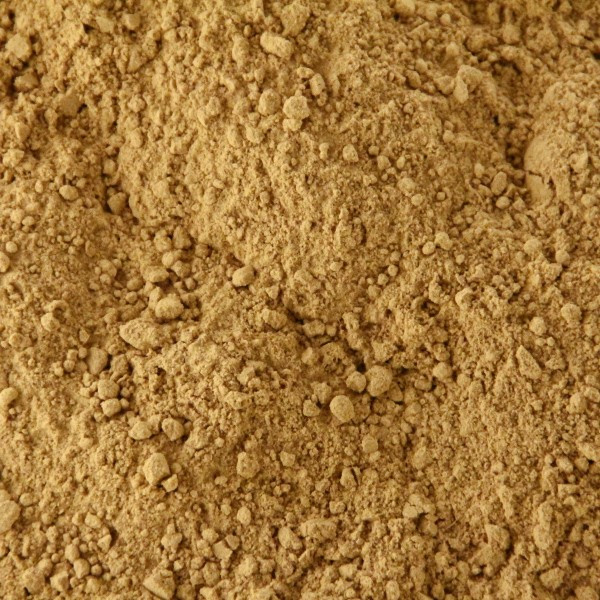
\includegraphics[width=0.3\linewidth]{imgs/spices/ginger-2.jpg}}
	% \hfill
	% \subfloat[\centering c]{\includegraphics[width=0.3\linewidth]{imgs/spices/ginger-3.jpg}}
	\caption{Ginger \taxon{}.}
	\label{fig:ginger_imgs}
\end{figure}

\subsection{The Botany of Ginger}

\subsection{The History of Ginger}

\subsection{The Names of Ginger}

\subsubsection{English}

\begin{etymology}\label{ety:ginger}
English \textit{ginger}, ca. 925
< reinforced by Old French \textit{gingivere, gingibre } `ginger'
< Medieval Latin \textit{gingiber} `ginger'
< Latin \textit{zingiber} `ginger'
< Ancient Greek {\gr{ζιγγίβερις}} \textit{ziggiberis} `ginger'
< Pali \textit{siṅgivera } `ginger'; cf. cognates Sanskrit शृङ्गवेर \text{śṛṇgavera}
< Dravidian \textit{*cinki-wēr} `ginger', South dravidian nominal compound  from the etyma of Tamil and Malayalam \textit{iñci} (both with regular loss of an initial sibilant) + \textit{vēr} (Proto-Dravidian \textit{wēr}); the base of \textit{*cinki} is a loanword
< unknown \textit{?} `ginger', unidentified Southeast Asian language; cf. cognates Khasi \textit{sying} /sʔiŋ/, Thai \textit{khing}, Vietnamese \textit{gừng}, Chinese \textit{jiāng}
<\textss{?} Proto-Sino-Tibetan \textit{*kjaŋ} `ginger'\footnote{\textcite{oed, ross_ginger_1952}; \textcite[5]{krishnamurti_dravidian_2003}; }
\end{etymology}

\begin{table}[!ht]
    \caption{Various names for ginger in English.}
\centering
\begin{tabularx}{\textwidth}{@{}l>{\itshape \small}lL>{\small}l@{}}
\toprule
\textbf{\#} & \multicolumn{1}{l}{\textbf{Species}} & \multicolumn{1}{l}{\textbf{Name}} & \multicolumn{1}{l}{\textbf{Source}} \\
\midrule
1	& Zingiber officinale	& black ginger	& \textcite{oed} \\
\textbf{2}	& \textbf{Zingiber officinale}	& \textbf{ginger}	& \textbf{\textcite{van_wyk_culinary_2014}} \\
3	& Zingiber officinale	& ginger root	& \textcite{oed} \\
4	& Zingiber officinale	& ginger spice	& \textcite{oed} \\
5	& Zingiber officinale	& green ginger	& \textcite{oed} \\
6	& Zingiber officinale	& white ginger	& \textcite{oed} \\
\bottomrule
\end{tabularx}
\label{table:names_ginger_en}
\end{table}



\subsubsection{Arabic}

\begin{etymology}\label{ety:zanjabil}
\textbf{Arabic} {زنجبيل} \textit{zanjabīl} `ginger', 609-632
< \textbf{Classical Syriac} {ܙܢܓܒܝܠ} \textit{zangabīl} `ginger'
< \textbf{Pahlavi} \textit{singibēr} `ginger', or via another Middle Iranian language
< \textbf{Sauraseni Prakrit} {𑀲𑀺𑀁𑀕𑀺𑀯𑁂𑀭} \textit{siṃgivera} `ginger'
<\textss{?} \textbf{Sanskrit} {शृङ्गवेर} \textit{śṛṅgavera} `ginger'
< \textbf{Dravidian} \textit{*cinki-wēr} `ginger', South dravidian nominal compound  from the etyma of Tamil and Malayalam \textit{iñci} (both with regular loss of an initial sibilant) + \textit{vēr} (Proto-Dravidian \textit{wēr}); the base of \textit{*cinki} is a loanword
< \textbf{unknown language} \textit{?} `ginger', unidentified Southeast Asian language; cf. cognates Khasi \textit{sying} /sʔiŋ/, Thai \textit{khing}, Vietnamese \textit{gừng}, Chinese \textit{jiāng}
<\textss{?} \textbf{Proto-Sino-Tibetan} \textit{*kjaŋ} `ginger'\footnote{\textcite{cal}; \textcite[90]{ciancaglini_iranian_2008}; \textcite[5]{krishnamurti_dravidian_2003}; \textcite{oed}}
\end{etymology}

\begin{table}[!ht]
\centering
\begin{tabularx}{\textwidth}{@{}l>{\itshape \small}lr>{\itshape}lL>{\small}l@{}}
\toprule
\textbf{\#} & \multicolumn{1}{l}{\textbf{Species}} & \multicolumn{1}{l}{\textbf{Name}} & \multicolumn{1}{l}{\textbf{Tr.}} & \multicolumn{1}{l}{\textbf{Gloss}} & \multicolumn{1}{l}{\textbf{Source}} \\
\midrule
1	& Zingiber officinale	& جنزبيل	& janzabīl	& 	& \textcite{wehr_dictionary_1976} \\
\textbf{2}	& \textbf{Zingiber officinale}	& \textbf{زنجبيل}	& \textbf{zanjabīl}	& \textbf{}	& \textbf{\textcite{wehr_dictionary_1976}} \\
\bottomrule
\end{tabularx}
\caption{Various names for ginger in Arabic.}
\label{table:names_ginger_ar}
\end{table}



\subsubsection{Chinese}

\begin{etymology}\label{ety:jiang}
\textbf{Mandarin Chinese} \traditionalchinesefont{薑} \textit{jiāng} `ginger', -221
< \textbf{Old Chinese} {䕬} OC /*kaŋ/ `ginger'
< \textbf{Proto-Sino-Tibetan} \textit{*kjaŋ} `ginger'; cf. Burmese ချင်း \textit{hkyang:}\footnote{}
\end{etymology}

\begin{table}[!ht]
\centering
\begin{tabularx}{\textwidth}{@{}l>{\itshape \small}ll>{\itshape}lL>{\small}l@{}}
\toprule
\textbf{\#} & \multicolumn{1}{l}{\textbf{Species}} & \multicolumn{1}{l}{\textbf{Name}} & \multicolumn{1}{l}{\textbf{Tr.}} & \multicolumn{1}{l}{\textbf{Gloss}} & \multicolumn{1}{l}{\textbf{Source}} \\
\midrule
1	& Zingiber officinale	& \tradchinesefont{幹薑}	& gānjiāng	& dry-ginger	& \textcite{defrancis_abc_2003} \\
\textbf{2}	& \textbf{Zingiber officinale}	& \textbf{\tradchinesefont{薑}}	& \textbf{jiāng}	& \textbf{ginger}	& \textbf{\textcite{kleeman_oxford_2010}} \\
3	& Zingiber officinale	& \tradchinesefont{鮮薑}	& xiānjiāng	& fresh-ginger	& \textcite{defrancis_abc_2003} \\
\bottomrule
\end{tabularx}
\caption{Various names for ginger in Chinese.}
\label{table:names_ginger_zh}
\end{table}



\subsubsection{Summary}

\begin{table}[!ht]
\centering
\begin{tabularx}{\textwidth}{@{}ll>{\itshape}lLl>{\small}l@{}}
\toprule
\textbf{\#} & \textbf{Language} & \multicolumn{1}{l}{\textbf{Term}} & \textbf{Gloss} & \textbf{Loan} & \multicolumn{1}{l}{\textbf{Source}} \\
\midrule
1	& English	& black ginger	& 	& no	& \textcite{oed} \\
2	& English	& ginger	& 	& yes	& \textcite{oed} \\
3	& English	& ginger root	& 	& no	& \textcite{oed} \\
4	& English	& ginger spice	& 	& no	& \textcite{oed} \\
5	& English	& green ginger	& 	& no	& \textcite{oed} \\
6	& English	& white ginger	& 	& no	& \textcite{oed} \\
\midrule
1	& Arabic	& janzabīl	& 	& yes	& \textcite{wehr_dictionary_1976} \\
2	& Arabic	& zanjabīl	& 	& yes	& \textcite{wehr_dictionary_1976} \\
\midrule
1	& Chinese	& gānjiāng	& dry-ginger	& no	& \textcite{defrancis_abc_2003} \\
2	& Chinese	& jiāng	& ginger	& no	& \textcite{kleeman_oxford_2010} \\
3	& Chinese	& xiānjiāng	& fresh-ginger	& no	& \textcite{defrancis_abc_2003} \\
\bottomrule
\end{tabularx}
\caption{Conventionalized names for ginger in English, Arabic, and Chinese, found in dictionaries.}
\label{table:names_ginger}
\end{table}










% EE:
% hot spicy root. XIII. ME. gingivere, repr. a conflation of OE. ġinġifer(e), ġinġiber (directly — medL.) with OF. gingi(m)bre (mod. gingembre) — medL. gingiber, zingeber, L. zingíber(i) — Gr. ziggiberis — Prakrit siṃgabera — Skr. śṛṇgavera-.
% Hence vb. flavour with ginger; treat (a horse) with ginger, (hence gen.) spirit up. XIX.

% OE:
% mid-14c., from Old English gingifer, gingiber, from Late Latin gingiber, from Latin zingiberi, from Greek zingiberis, from Prakrit (Middle Indic) singabera, from Sanskrit srngaveram, from srngam "horn" + vera- "body," so called from the shape of its root. But this may be Sanskrit folk etymology, and the word may be from an ancient Dravidian word that also produced the Malayalam name for the spice, inchi-ver, from inchi "root."

% The word apparently was readopted in Middle English from Old French gingibre (12c., Modern French gingembre). In reference to coloring, by 1785 of fighting cocks, 1885 of persons (gingery with reference to hair is from 1852). Meaning "spirit, spunk, temper" is from 1843, American English (see gin (v.1)). Ginger-ale is recorded by 1822, the term adopted by manufacturers to distinguish their product from ginger beer (1809), which was sometimes fermented. Ginger-snap as a type of hard cookie flavored with ginger is from 1855, American English.

% MW:
% Middle English ginger, gingere, alteration of gingivere, alteration (influenced by Old French gingembre, gingibre ginger, from Medieval Latin gingiber) of Old English gingifer, modification of Medieval Latin gingiber, alteration of Latin zingiber, from Greek zingiberi, probably modification of Sanskrit śṛngavera
% First Known Use: before 12th century (sense 1)

% AH:
% [Middle English gingivere, from Old English gingifer and from Old French gingivre, both from Medieval Latin gingiber, from Latin zingiberi, from Greek zingiberis, of Middle Indic origin (akin to Pali singiveram), from Dravidian : akin to Tamil iñci, ginger (of southeast Asian origin) + Tamil vēr, root.]

%wk
%From Middle English gingere, alteration of gingivere, from Old English gingifer, gingiber (influenced by Old French gingembre), from Medieval Latin gingiber, zingiber, from Latin zingiberi, from Late Ancient Greek ζιγγίβερις (zingíberis), from Sauraseni Prakrit (siṃgivera), from Sanskrit शृङ्गवेर (śṛṅgavera) (influenced by शृङ्ग (śṛṅga, “horn”)), ultimately from Proto-Dravidian *cinki-wēr. 
